\section{Assignment 2: Image Segmentation by $K-$means\ \ Clustering}
\label{sec:assignment2}

In this assignment we use K-means clustering for image segmentation. K-means clustering is a very simple but effective clustering algorithm, but it also comes with some drawbacks. We examine the strengths and weaknesses of this method applied to image segmentation.

\subsection{Problem definition}

Given an image, the goal is to divide it into disjoint regions. These regions should correspond to coherent areas in the image. In  a perfect result, each ``object'' is matched to exactly one region. What an ``object'' is, depends on the application: we might want to separate different colors or textures, or to separate the background from the foreground, or obtain a region for each physical object in the image. In this assignment we examine K-means clustering applied to image segmentation.
 In particular we:
\begin{itemize}[noitemsep]
	\item Implement K-means clustering.
	\item Study the influence of augmenting the color information with spatial information in the form of normalized pixel coordinates.
	\item Study the influence of the number of clusters chosen.
	\item Discuss the advantages and disadvantages of K-means clustering for image segmentation.
\end{itemize}

\subsection{Methodology}

\subsection{Overview}
K-means clustering is an algorithm used to cluster data. It works as follows: assume we have data $x_1,\ldots,x_N \in \mathbb{R}^n$. We first chose K centroids $\mu_k \in \mathbb{R}^n$ randomly. Then we assign each data point $x_i$ to the centroid $\mu_j$ which minimizes the distance between $x_i$ and the centroids $\mu_k$. To record this relation we use an indicator matrix $r(i,j) \in \{0,1\}$, with $r(i,j)=1$ if data point $x_i$ is assigned to centroid $\mu_j$ and $0$ otherwise. We can define an objective function, which the K-means clustering algorithm tries to minimize. For this we define the distortion as
\begin{equation}
	J = \sum_{n=1}^{N} \sum_{k=1}^{K} r(n,k) \left\|x_n-\mu_k\right\|^2.
\end{equation}
This is the sum of squared distances from each data point to its assigned centroid, and we want to minimize it. For this we use the following iterative K-means clustering method:
\begin{enumerate}
\item Initialize the $K$ centroids $\mu_k$ with random values.
\item Assign each data point $x_i$ to its nearest centroid $\mu_j$ and update the indicator matrix
\[
	r(i,j)= \begin{cases}
               1 \text{, if } j = \argmin_k\left\|x_i-\mu_k\right\| \\

             0 \text{ otherwise.}
            \end{cases}
\]
\item Calculate new centroids $\mu_k$ as the mean of all data points assigned to the k-th cluster, i.e. 
\[
	\mu_k = \frac{\sum\limits_{i=1}^N r(i,k) x_i}{\sum\limits_{i=1}^N r(i,k)}
\]
\item Calculate the distortion J with the new assignment and centroids and check for convergence. This is done by checking if the ratio of the old and new $J$ does not change any more, i.e if the ratio lies below a user given threshold. We use the absolute value of 1 minus the ratio, so that the algorithm can also make $J$ a little worse, as this could make the end result better. As long as J does not converge, repeat steps 2 to 4.
\end{enumerate} 

We use two different methods to get data points from pixel values. One is to just take the color values of each pixel, the other is to normalize each coordinate of a pixel to $[0, 1]$ and use the color value and the coordinate of the pixel, resulting in a 5-dimensional space.

To illustrate the results we can color each pixel in the image with the color of the associated centroid. Alternatively we can associate the clusters with mutually distinct colors and colorize the image using these, instead of the value of the centre. This helps to better see the cluster boundaries.

\subsection{Implementation}

You can run the image segmentation with the function \texttt{image\_segmentation(image\_path, K, precision, use\_coordinates, use\_distinct\_colors)}, where \texttt{image\_path} is the path to the image, \texttt{K} is number of clusters, \texttt{precision} is the precision used for the convergence criterion of the distortion, \texttt{use\_coordinates} is a boolean that says if coordinates should be used or not and \texttt{use\_distinctcolors} is a boolean that if true colors the result with distinct colors or the color of the cluster center otherwise. It returns the segmented image, colored with the chosen option, the cluster centroids and the indicator matrix.
 We will explain some details of the implementation in the next part.

To make use of vectorization and matrix operations we vectorize the image. That means instead of indexing pixels by two indexes we use just one. This has the advantage that the indicator matrix is a two dimensional matrix. Thus we have that $r(i,j)*\text{centroids}$, where centroids is the vector of centroids, gives the centroid associated with each data point. And if $X$ is the data matrix, i.e $X(i,:)$ is the i-th data point, then $r(i,j)^T * X$ gives the sum of all data points associated with one cluster.

As mentioned above we use $\vert 1-J_{old}/J_{new}\vert < \text{precision}$ as a convergence criterion, where we take absolute values to allow the objective value to also get a worse in the hope of not getting stuck in a local minimum.

One problem is that calculating the mean of the data of a cluster is not possible if the cluster is empty. This can happen in the assignment stage. To fix this, we choose for each empty cluster a random data point and remove this from its cluster and add it to the empty cluster.

The function distinguishable\_colors was taken from mathworks.com/matlabcentral/fileexchange and the relevant license is included.
\subsection{Experiments}

We analyzed K-means clustering for image segmentation with the test images \texttt{future.jpg}, \texttt{mm.jpg} and \texttt{simple.PNG}, and made the following experiments. First we clustered each image into 3 and 5 clusters, both with and without the use of coordinates. Then we separately examined the image \texttt{mm.jpg}. We used different K values and varied the use of coordinates. We also ran the algorithm several times on \texttt{simple.PNG} to show the effect of bad initialization.

In the figure \ref{fig:testimages} the test images are shown. The \texttt{future.jpg} images shows a drawn image. It contains only a restricted color palette. The test image \texttt{mm.jpg} is a photography of an advertisement screen. It has a lot of artifacts in the screen and many fine details in the background which makes segmentation more difficult. The third test image \texttt{simple.PNG} is a artificially generated image. It just contains 2 filled circles on an uniform background. It should be very easy to segment this image.
\begin{figure}[h!]
	
\includegraphics[width=0.38\linewidth]{figures/task2/future.jpg}
	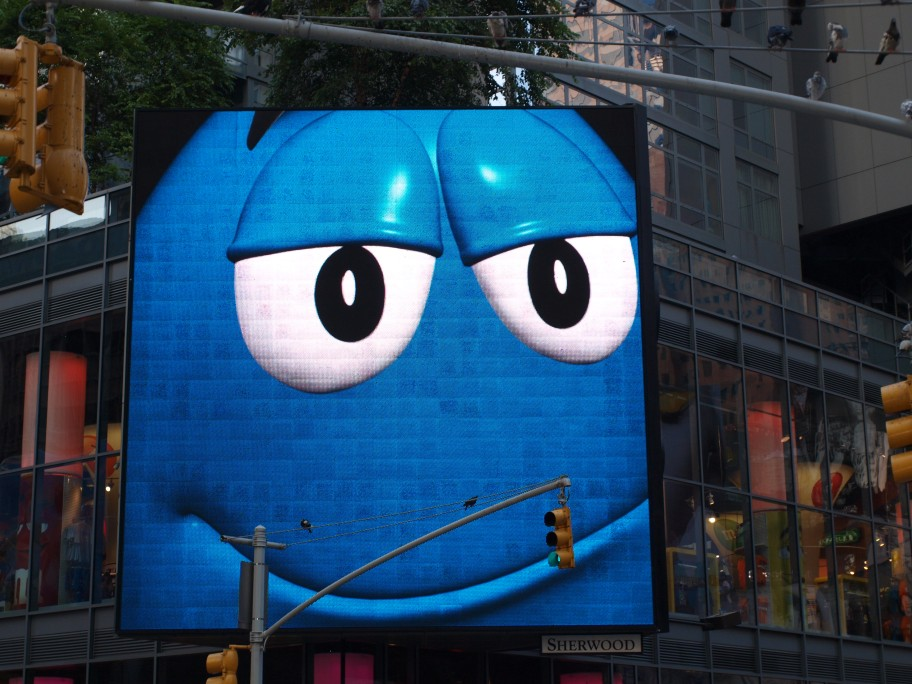
\includegraphics[width=0.398\linewidth]{figures/task2/mm.jpg}
	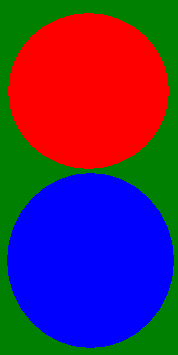
\includegraphics[width=0.15\linewidth]{figures/task2/simple.PNG}
	\caption{The 3 test images. From left to right: future, mm and simple.}
	\label{fig:testimages}
\end{figure}

\subsubsection{Influence of using coordinates}

Figures \ref{fig:future:coords}, \ref{fig:mm:coords} and \ref{fig:simple:coords} illustrate the result of the segmentation by coloring each pixel by the color value of its associated centroid. We show the influence of the usage of coordinates for K=3 and K=5 clusters for each test image.

\begin{figure}[h!]
\centering
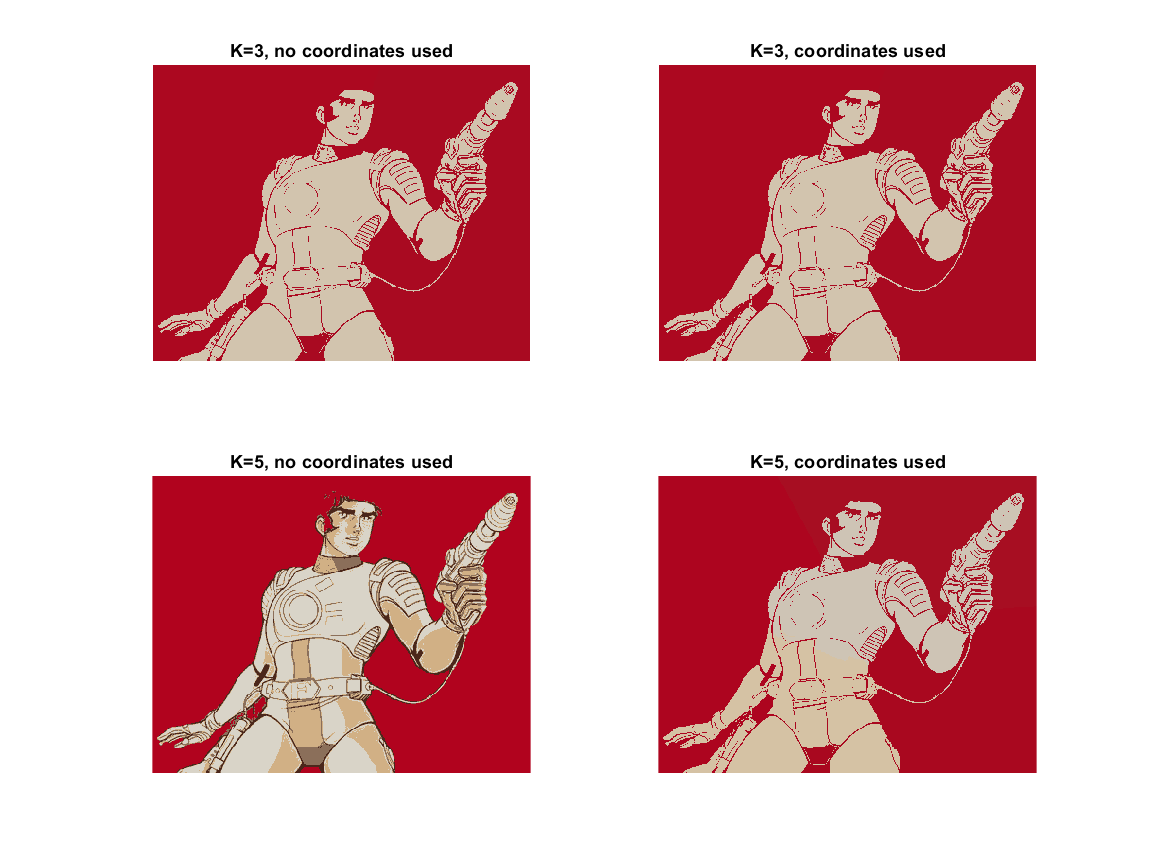
\includegraphics[width = 0.95\linewidth]{figures/task2/future_coordinates.png}
\caption{Coordinate experiment for \texttt{future.jpg}}
\label{fig:future:coords}
\end{figure}

The results for the image \texttt{future.jpg} are shown in figure \ref{fig:future:coords}. We can see that the segmentation without using coordinates produces a pleasing result. It can separate the different colors very accurately. This is the case as the image contains only a limited number of colors, and all colors in a coherent region have the same color. For the clustering with coordinates it appears that the algorithm found less clusters than K. This is the case as the background gets segmented into multiple regions. This happens, because the pixels on the right and on the left have on one hand the same color, but are spatially far apart, so it makes sense to split the background in a left region and right region. For $K=5$ the image gets split into 3 background region a top part of person region and a bottom part of person region. We can see that not only the color is important, but also the spacial relation. We can already see here, that using the colors of the cluster center makes the inspection of the result hard, as several cluster, in particular for the case which uses coordinates, can have the same or very similar colors.

\begin{figure}[h!]
\centering
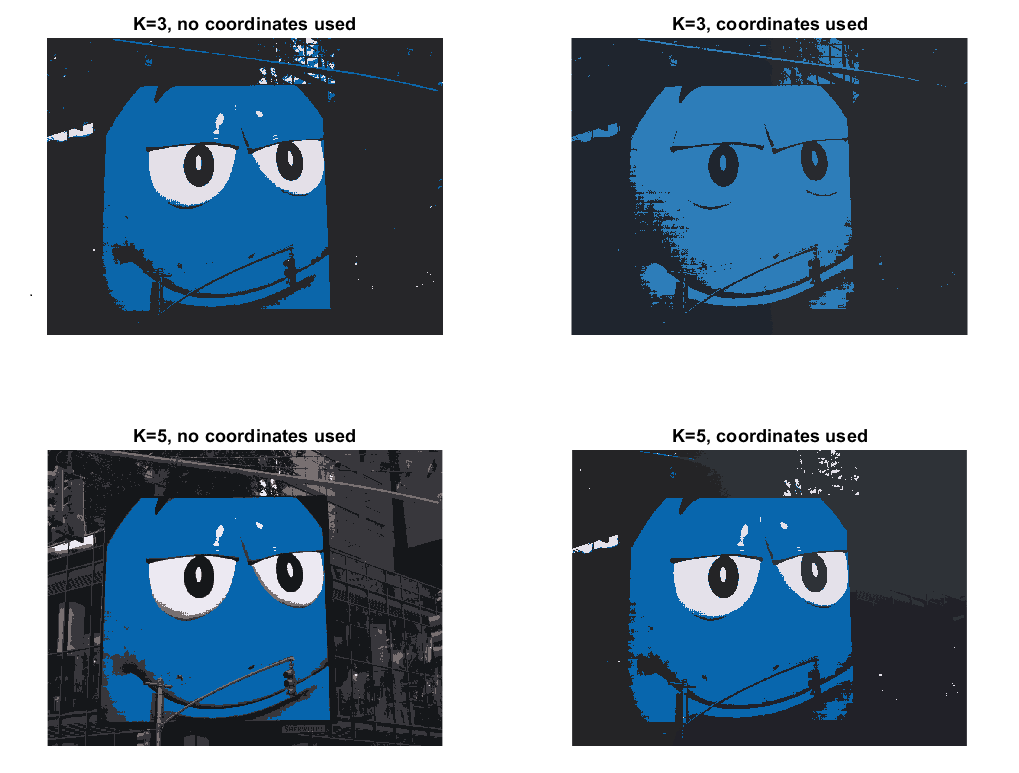
\includegraphics[width = 0.8\linewidth]{figures/task2/mm_coordinates.png}
\caption{Coordinate experiment for \texttt{mm.jpg}}
\label{fig:mm:coords}
\end{figure}

The results for the image \texttt{mm.jpg}, shown in figure \ref{fig:mm:coords}, are hard to interprete, because we can't really see the different clusters, as they have very similar colors and we will explain this later. Therefore we repeated the experiment for $K=5$ and used distinct colors. The result is shown in figure \ref{fig:mm:coords:distinct}. 

We see that for $K=3$ without coordinates it separated the image into a white, black and blue region. With the use of coordinates it again separated the image into a blue foreground region and 2 background regions. As the average of the background is everywhere similar we can't see the different clusters. For K=5 it separated the image into 5 colors. as only the color is important, we can see a lot of fine details in the background, on the other hand if we use coordinates the fine details aren't preserved, as they don't form a connected region. K-means basically produces a Voronoi tessellation of the space. Therefor the regions should be polygons or circles. If we use distinct colors we can clearly see in figure \ref{fig:mm:coords:distinct}, that only using colors produces very spatially irregular structures, as they are only defined by color and not their spacial relation. On the other hand, if we use coordinates the algorithm produces spatially regular regions. Only on the border between two regions irregularities can occur, as at that position color is more important, because the distance in spatial domain to the two centers is equal.

\begin{figure}[h!]
\centering
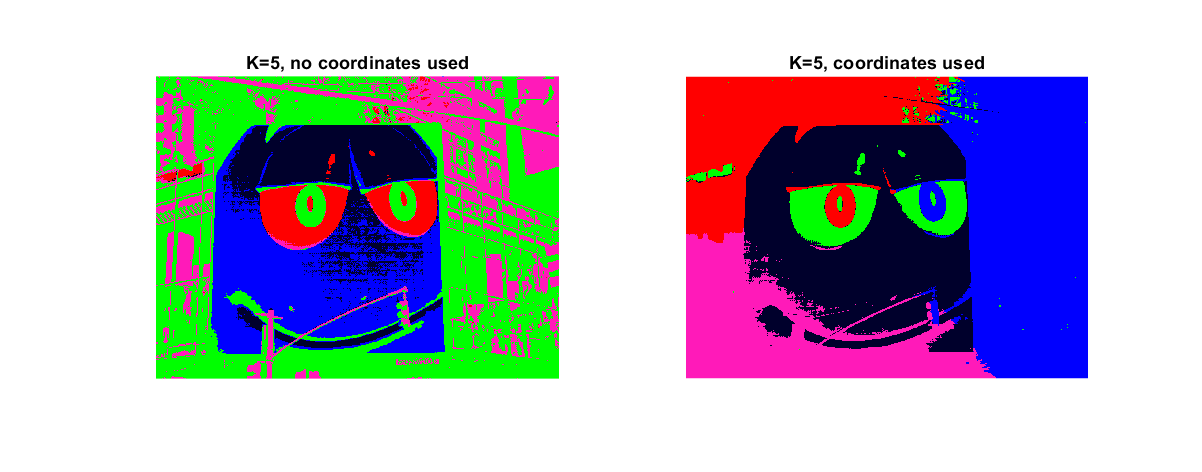
\includegraphics[width = 0.9\linewidth]{figures/task2/mm_bad_visibility.png}
\caption{Coordinate experiment for \texttt{mm.jpg} with distinct colors.}
\label{fig:mm:coords:distinct}
\end{figure}

The clustering algorithm has no problem segmenting an image like \texttt{simple.PNG}. For $K=5$ the algorithm has to produce too many clusters. Without spatial information it just creates two extra clusters containing only a single pixel. With spatial information, it divides two of the cluster into a left and right part, or top and bottom part.

\begin{figure}[h!]
\centering
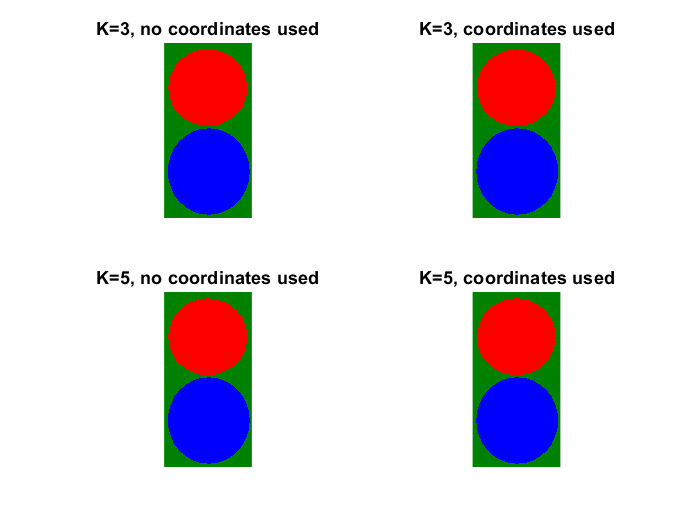
\includegraphics[width = 0.7\linewidth]{figures/task2/simple_coordinates.png}
\caption{Coordinate experiment for \texttt{simple.PNG}}
\label{fig:simple:coords}
\end{figure}

\subsection{Experiment with the number of clusters}
In a second experiment we took the picture \texttt{mm.jpg} and segmented it using different number of coordinates once without coordinates and once with. The results are shown in figure \ref{fig:mm:nocoords:manyK} and \ref{fig:mm:coords:manyK}. We used distinct colors to color the cluster to better see the resulting cluster.

\begin{figure}[h!]
\centering
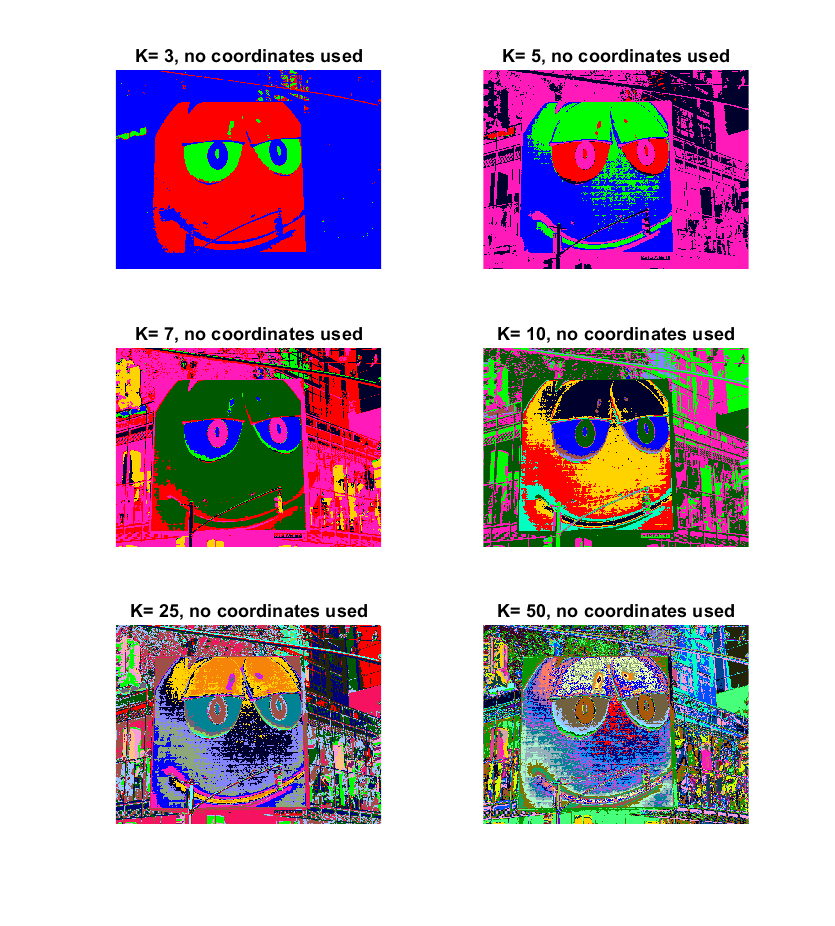
\includegraphics[width =0.8\linewidth]{figures/task2/mm_nocoords_manyK.png}
\caption{Clustering with different values of K without use of coordinates}
\label{fig:mm:nocoords:manyK}
\end{figure}

We see different trends. First, we see that without coordinates the clusters get more and more irregular. We can see that the more clusters we take, the less one cluster corresponds to a physical object. This is because an object consists of many, although similar, colors and as the spatial relation is missing, the algorithm can't know which regions should belong together. If we would color the image with the cluster centroids, the result would be visually similar to the original picture and this could be used for image compression. We can also see that for a relatively low number of clusters the fine details in the background, like windows or the scaffolding is preserved, but for higher numbers such details disappear and the cluster more closely resemble noise.

\begin{figure}[h!]
\centering
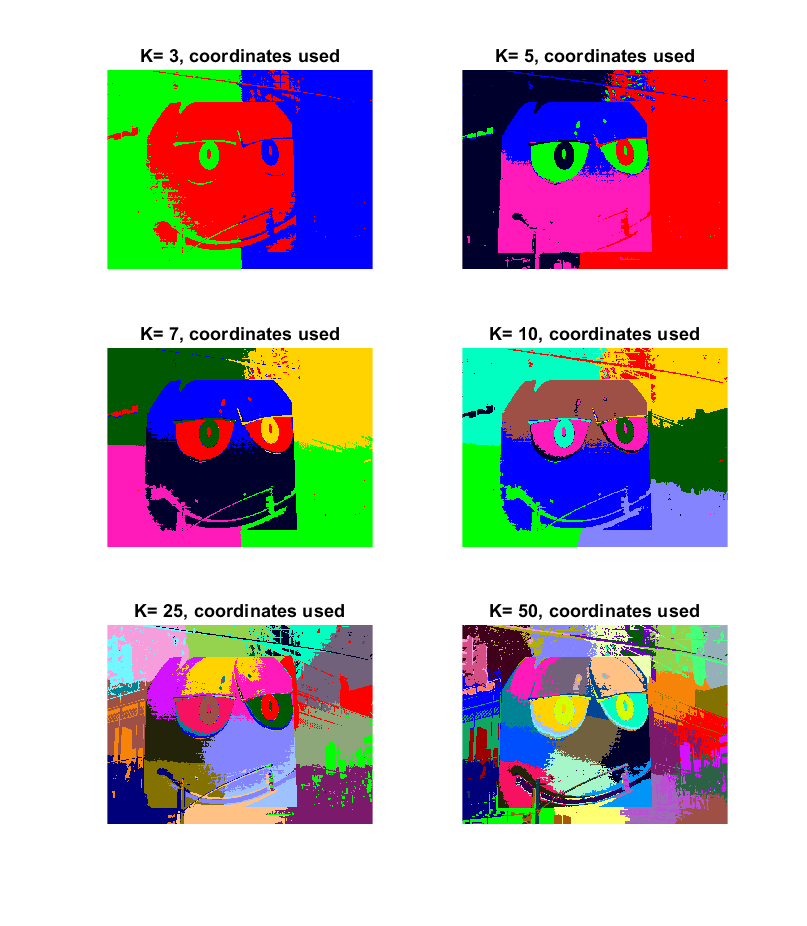
\includegraphics[width =0.8\linewidth]{figures/task2/mm_coords_manyK.png}
\caption{Clustering with different values of K without use of coordinates}
\label{fig:mm:coords:manyK}
\end{figure}

For the case with coordinates, shown in figure \ref{fig:mm:coords:manyK}, we see the algorithm tends to produce spatially connected regions. Here we can also see the splitting of the regions to multiple cluster as the number of clusters increases, as mentioned above in. We see that the coordinates force the region to become more like closed polygons. This makes it impossible to segment spatially irregular structures like the scaffolding and windows, even if we take a very large number of clusters. 

\section{Discussion}
It is immediate clear that the main strength of the K-means clustering algorithm is that it uses no domain knowledge. We could just take this general algorithm and apply it to image segmentation, giving even useful results. So it can be very useful to use K-means clustering as a baseline method to compare other methods against. It is also a very simple algorithm and we can just use more features if we wish to have a more accurate result, where accurate naturally depends on the application.

We also see in our experiments that using coordinate information or not depends mostly on the application. If we want to compress an image by using only a handful of colors, using just color information is much better. Also if we are interested in non polygonal structures, not using coordinates can lead to better results. But if we have a large number of clusters and don't use coordinates the different cluster correspond less and less to semantically coherent regions. If we use coordinates, we get spatially connected regions. This can be useful in some applications. One could imagine that we could post-process an image which was segmented with K-means clustering using many clusters by merging clusters that are very similar, based on some metric. This metric could use other features.

One main disadvantage is that the result can vary a lot with different initializations. We could circumvent this by using a deterministic initialization. Moreover for every pixel the distance to every cluster has to be calculated. We can see this in figure \ref{fig:simple:badinit}. This can be computationally expensive for large images or large number of clusters. Moreover there is no guarantee that the distortion doesn't end up in a local minimum. Moreover as the results strongly depends on the initialization, we get a different result each time we run the algorithm. This could be bad as we can't know which clusters corresponds to which part of the image, without looking at the result. This makes the performance of the algorithm unpredictable.

\begin{figure}[h!]
\centering
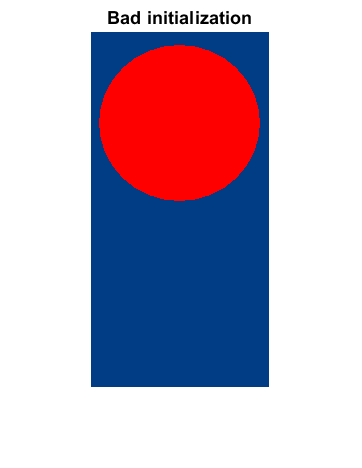
\includegraphics[width =0.5\linewidth]{figures/task2/bad_initialization.png}
\caption{Clustering with different values of K without use of coordinates}
\label{fig:simple:badinit}
\end{figure}